
\documentclass[a4paper,12pt]{article}
%%%%%%%%%%%%%%%%%%%%%%%%%%%%%%%%%%%%%%%%%%%%%%%%%%%%%%%%%%%%%%%%%%%%%%%%%%%%%%%%%%%%%%%%%%%%%%%%%%%%%%%%%%%%%%%%%%%%%%%%%%%%%%%%%%%%%%%%%%%%%%%%%%%%%%%%%%%%%%%%%%%%%%%%%%%%%%%%%%%%%%%%%%%%%%%%%%%%%%%%%%%%%%%%%%%%%%%%%%%%%%%%%%%%%%%%%%%%%%%%%%%%%%%%%%%%
\usepackage{eurosym}
\usepackage{vmargin}
\usepackage{amsmath}
\usepackage{graphics}
\usepackage{epsfig}
\usepackage{framed}
\usepackage{subfigure}
\usepackage{fancyhdr}
\usepackage{framed}
\usepackage{subfiles}
\usepackage{graphics}
\usepackage{newlfont}
\usepackage{eurosym}
\usepackage{amsmath,amsthm,amsfonts}
\usepackage{amsmath}
\usepackage{enumerate}
\usepackage{color}
\usepackage{multicol}
\usepackage{amssymb}
\usepackage{multicol}
\usepackage[dvipsnames]{xcolor}
\usepackage{graphicx}

\setcounter{MaxMatrixCols}{10}
%TCIDATA{OutputFilter=LATEX.DLL}
%TCIDATA{Version=5.00.0.2570}
%TCIDATA{<META NAME="SaveForMode"CONTENT="1">}
%TCIDATA{LastRevised=Wednesday, February 23, 201113:24:34}
%TCIDATA{<META NAME="GraphicsSave" CONTENT="32">}
%TCIDATA{Language=American English}


\pagestyle{fancy}
\setmarginsrb{20mm}{0mm}{20mm}{25mm}{12mm}{11mm}{0mm}{11mm}
\lhead{MA4128} \rhead{Mr. Kevin O'Brien}
\chead{Advanced Data Modelling}
%\input{tcilatex}
%http://www.electronics.dit.ie/staff/ysemenova/Opto2/CO_IntroLab.pdf
\begin{document}
\section*{Two Table Operations: SQL Joins}	
The following code should set up four dataframes, 3 for the first exercise, and another one for the second.
\begin{framed}
\begin{verbatim}
library(dplyr)
#########

PID <- c(101,102,103,104,105,106,107,108,110)
VarA <- sample(letters[1:12],length(PID),replace=T)
VarB <- sample(10:20/10,length(PID),replace=T)
Table1 <- data.frame(PID,VarA,VarB)
rm(PID);rm(VarA);rm(VarB);

PID <- c(101,102,103,104,105,106,108,109)
Var1 <- sample(c("RAVC","SLIR","HUFP","GRFD"),length(PID),replace=T)
Var2 <- sample(9:16,length(PID),replace=T)
Table2 <- data.frame(PID,Var1,Var2)
rm(PID);rm(Var1);rm(Var2);


PrimKey <- c(101,102,103,104,105,106,107,108,109,110)
X1 <- c("Dog","Cat","Dog","Dog","Duck","Cat","Dog","Cat","Hamster","Goat")
X2 <- c("BodyRolls","BodyRolls","Hikicks","Hikicks","BodyRolls",
        "BodyRolls","Hikicks","Hikicks","BodyRolls","BodyRolls")
Table3 <- data.frame(PrimKey,X1,X2)
rm(PrimKey);rm(X1);rm(X2);

#########

Species <- c("Setosa","Versicolor","Virginica")
Country <- c("France","Scotland","Ireland")
iris1 <- sample_frac(iris,0.95)
iris2 <- data.frame(Species,Country)
\end{verbatim}
\end{framed}
\newpage
\begin{figure}[h!]
	\centering
	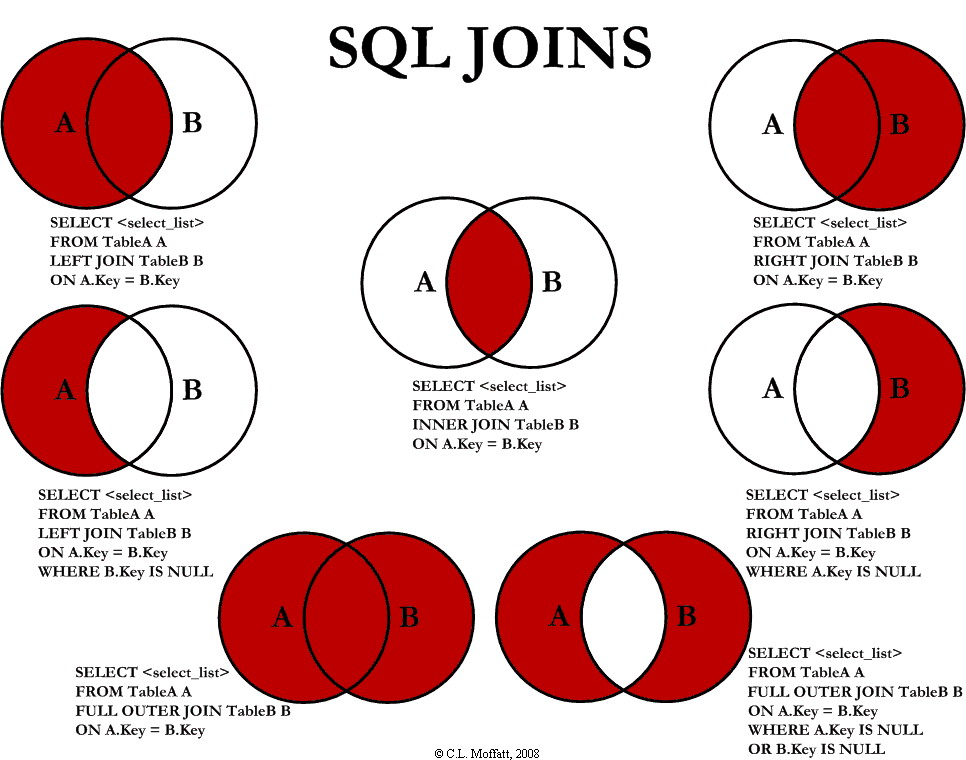
\includegraphics[width=0.7\linewidth]{SQLjoins}
	\caption{}
	\label{fig:sqljoins}
\end{figure}

\end{document}